% !TeX root = ../../../Main.tex
\chapter{Solution Methods for Markov Decision Processes}
\label{chapter2}

\section{Markov Decision Process}

Path planning through calm air can be done analyzing how a glider behaves in calm air. Flying a glider can be regarded as a decision process where the pilot decides what control surface position is suitable for the current situation. By varying, for example, the elevator position, the pilot can control the speed of the glider and thereby the flight path angle. In reality, this process is time-continuous. Computers - however - can only deal with discrete processes. Therefore it is common practice to introduce a time step $\Delta t$. At each moment in time $t_k = t_0 + k\Delta t$, an elevator position is chosen and is kept constant until $t_{k+1}$. The smaller the time step, the better the approximation of a continuous process. Each state $s_t$ in this decision process has the Markov property, i.e. the information needed to calculate $s_{t+1}$ is fully contained in $s_t$. In other words, the probability of reaching a state $s_{t+1}$ by taking an action $a_t$ only depends on the state $s_t$. The predecessor states of $s_t$ are irrelevant for $P(s_{t+1}|s_t,a_t)$. A decision process where the Markov property applies to all states is called a Markov Decision Process (MDP)\nomenclature[A]{MDP}{Markov Decision Process}. 

\begin{align}
P(s',r|s,a)&=\mathbb{P}[s_{t+1}=s',r_{t+1}=r|s_t=s,a_t=a] \\
&= \mathbb{P}[s_{t+1}|s_t,a_t,s_{t-1},a_{t-1},s_{t-2},a_{t-2},...]
\end{align}

\section{The Principle of Optimality}
\label{sec:optimality}

According to Bellman's principle of optimality, the solution of some optimization problems can be put together from the solution of subproblems. This is the basis for all dynamic programming algorithms. If an agent chooses the optimal action in a state $s_t$ and all states it visits afterwards ($s_k$, $k=t+1, t+2, ...,T$) , the resulting trajectory is the optimal one from $s_t$ to the terminal state $s_T$.

The principle of optimality can be expressed by the Bellman Equation, which is shown in section~\ref{sec:Bellman_Equation}. Prior to introducing the Bellman Equation, a few necessary concepts and terms are explained in the following sections.

(Bsp. Fibonacci Folge und/oder shortest path)

\section{The Agent - Environment System}

In Reinforcement Learning scenarios, an agent interacts with its environment and thereby learns how to maximize some sort of scalar reward signal. The agent aims to maximize its total reward by choosing - at each time step - the best possible action $a$ from a set of actions $\mathcal{A}$. 
The agent has no prior knowledge about the environment and about how to behave in an optimal way. Instead, it learns by interacting with its environment and the information it receives during training. Before each step, the agent is in a state $s_t$, chooses an action $a_t$ and receives a scalar reward $r_t$ and an observation $o_t$ representing the next state $s_{t+1}$. The process is repeated, then. Figure \ref{fig:agent_env_system} illustrates what happens at each time step. Note that, unlike in this thesis, a timestep is denoted by an index $k$ instead of $t$. The observation $o_t$ can just be $s_{t+1}$. However, in partially observable environments, it might only be a part of $s_{t+1}$ or any information regarding the true state $s_{t+1}$. In this work, $o_t$ is equal to $s_{t+1}$ (i.e. the agent has complete knowledge about his state at any time).

The reward $r_t$ the agent receives at each step is determined by a reward function $\mathcal{R}(s,a)$. The reward function maps from states (and sometimes actions) to a scalar reward and characterizes the mission target. The choice of a reward function is crucial for the success of any RL-based trajectory optimization algorithm. The only way to "tell" the agent, what his goal is, is by defining the reward function. 

Generally, a reward function should guide the agent to the target. There are, however, restrictions on what a reward function should contain. If too much information about the problem is put into the reward function, this might lead to a suboptimal result. If, for example, a user trying to solve an MDP thinks a specific terminal state might be better than the others, he might be tempted to increase the final reward for reaching this - seemingly optimal - terminal state. But any (unnecessary) assumption, that is put in the reward function, can restrict the agent's ability to find an optimal trajectory on his own. A false assumption can sometimes even jeopardize convergence of the whole algorithm. Therefore, a good reward function should only give a reward for reaching a target state and penalize every step the agent does, if time is crucial. It can also penalize any step that leads to an undesired terminal state (in this work, touching the ground is such a case). This way, the agent can find a good trajectory without restrictions. More on the reward function used here can be found in section \ref{sec:reward-function}.

\begin{figure}[h]
	\centering
	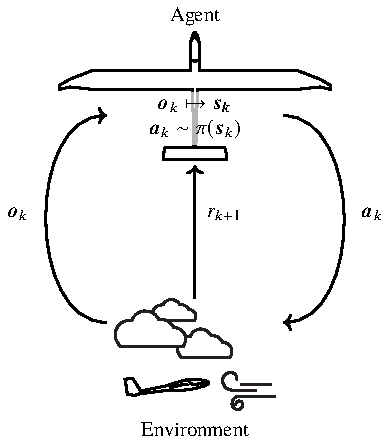
\includegraphics[width=0.5\textwidth]{src/pics/RLProblem.pdf}
	\caption{The Agent-Environment-System~\cite{Notter2018}}
	\label{fig:agent_env_system} 
\end{figure}

\section{Model Based and Model Free Learning}
\label{sec:modelbasedmodelfree}

MDP solution methods can be divided into model-free and model-based methods. In model-based methods, the agent uses a model to predict the reaction of the environment to any of his actions. An environment model typically takes a state-action pair and returns the next state and next reward. If the environment is discrete and stochastic, there are multiple possible next states and rewards.\footnote{In a continuous stochastic environment, there would be a distribution of successor states and rewards.} A \textit{sample model} returns one of the possibilities, whereas a \textit{distribution model} returns some representation of all possible next states and rewards. To distinguish experience from a model from real experience, the results from a model are referred to as \textit{simulated experience}~\cite[section~8.1]{SuttonBarto2018}.

Regardless of the type, all models approximate what might happen to the agent in future time steps. Whether the experience gathered through a model is useful obviously depends on its quality. Every model adds complexity to an algorithm. The more complexity, the higher the cost of implementing and updating it. Model free methods are generally simpler to implement and more scalable. 

In model free solution methods, there is no model of the environment. The agent is not explicitly aware of the environment behavior. Instead, the policy (and value function) are directly affected by the experience of the agent. Sutton and Barto refer to model free methods as some sort of "trial and error" (c.f. \cite[section~1.5]{SuttonBarto2018}). If the goal is to maximize the expected return, a model might not be needed at all. In TRPO, for example, the policy is optimized by maximizing the expected return with respect to the policy parameters $\theta$ by sampling trajectories through the state space and utilizing a gradient based optimization method. This is simpler than learning a model of the environment and using it to plan.

A model of the environment is - in principle - not required for successful training. It can however be used to gather simulated experience (c.f. section \ref{sec:modelbasedmodelfree}) and therefore reduce training time on a real agent like a robot. Although imperfect, information from a model can be useful in such cases where training time is restricted which particularly holds true for robots flying outdoors.

For more information on how machine learning algorithms can be classified, please refer to chapter \ref{chapter3}, which also contains one classification example in Fig. \ref{fig:classification_ml}.

\section{Agent}

The agent in an MDP consists of at least one of the following parts.

\begin{itemize}
	\item Policy: \\
	A mapping from states to actions that tells the agent what to do (c.f. section \ref{sec:policy})
	\item Value Function: \\
	A mapping from states (or state-action pairs) to values (c.f. section \ref{sec:value-function})
	\item Model: \\
	A model of the environment that might be updated by the agent's experience
\end{itemize}

Most agents implement a policy. They also can have a value function, like in actor-critic algorithms, where the value function is used for so called bootstrapping \footnote{Bootstrapping is a general term, that applies to methods, that make use of previous results in order to obtain another one. In this case, it means utilizing the Bellman Expectation Equation to estimate the return $G_t$ by doing a one step lookahead. The state value $V(s)$ is then updated utilizing $V(s')$, which can be seen as a "previous" result.}.

\begin{align}
\mathbb{E}[G_t|s_t=s] &= \mathbb{E}[r_{t+1} + \gamma G_{t+1}|s_t=s, a_t=a] \\
&=\mathbb{E}[r_{t+1}+ \gamma V(s_{t+1})|s_t=s, a_t=a]
\end{align}

Instead of sampling a complete episode, bootstrapping makes it possible to learn from incomplete episodes.

\section{Return}

The return $G_t$ at a time step $t$ is the cumulative reward $r_t$ at each step from the state $s_t$ onwards until reaching a terminal state:

\begin{equation}
G_t = \sum_{k=0}^{T-t-1}\gamma^k r_{t+k+1}
\end{equation}

If $\gamma \in (0,1]$ is close to zero, immediate rewards are weighted stronger. If $\gamma$ is close to one, rewards in the distant future are weighted likewise, making decisions more far sighted. In infinite horizon problems, where there is no terminal state, $\gamma$ must be less than one in order to avoid infinite returns. In finite horizon (i.e. episodic) MDPs, $\gamma$ is usually close to, or exactly one.

Each decision at a given state $s_t$ also affects what the next state $s_{t+1}$ is and therefore the next reward. More on the reward and what role it plays in Dynamic Programming is explained in section \ref{sec:reward-function}.

\section{Policy}
\label{sec:policy}
In reinforcement learning problems, a policy is usually the part that represents the agent. It contains all the information needed to decide what action to choose in each state the agent visits. A policy is a mapping from states to actions.

Generally, a policy is a mapping from states to actions. A policy can also be stochastic, in which case it maps from states and actions to a number between 0 and 1, which represents the probability to pick $a$ when in $s$.

\begin{equation}
\pi: \mathcal{S} \times \mathcal{A} \mapsto [0,1]
\end{equation} 

If the policy is deterministic, only one $a_t$ out of $\mathcal{A}$ has a probability of one with all other actions assigned to probability zero. In any policy, the sum of all possible action-probabilities must be one.

\begin{equation}
\pi(a|s) = \mathbb{P}[a_t=a|s_t=s]
\end{equation}

This yields equations \ref{eq:transprobpi} and \ref{eq:rewardpi} for the state transition probability and the reward function under policy $\pi$. The reward function is explained in section \ref{sec:reward-function}.

\begin{equation}
\mathcal{P}_\pi(s,s')=\sum_a \pi(a|s)\mathcal{P}(s'|s,a)
\label{eq:transprobpi}
\end{equation}
\begin{equation}
\mathcal{R}_\pi(s) = \sum_a\pi(a|s)\mathcal{R}(s,a)
\label{eq:rewardpi}
\end{equation}

At each timestep, the agent receives a state observation $o_{t-1}$ from the environment, passes it to the policy and the policy returns an action $a_t$. This action is taken and the agent gets a new observation $o_t$ and a reward $r_t$. This process is repeated until the agent reaches a terminal state.

A policy can be implemented in many different ways. The simplest option is a table where each field contains the action for one state or - if the policy is stochastic - all possible actions and their respective probabilities. Other examples include linear combinations of the inputs and linear combinations of basis functions. The most popular way to implement a policy is - however - through an artificial neural network (ANN). More information about neural networks is given in chapter \ref{chapter4}.  

\section{Value Functions}
\label{sec:value-function}

Some RL-algorithms try to find a policy directly from experience. Others, like Q-learning, additionally utilize a so called value function. A value function maps from states or state-action pairs to their values. In this context, the value of a state or an action is a measure of how useful it is for the agent to visit the respective state or choosing the respective action. There are two types of value functions, state value functions and action value functions. The state value $V(s)$ is the expected total return from state $s_t$ onwards until the episode terminates. The action value also takes into account what the agent chooses to do in state $s_t$. It is the expected total return from state $s_t$ when choosing action $a_t$.

\begin{equation}
V(s) = \mathbb{E}[G_t|s_t=s]
\label{eq:state_value_fun}
\end{equation}

\begin{equation}
Q(a|s) = \mathbb{E}[G_t|s_t=s,a_t=a]
\label{eq:action_value_fun}
\end{equation}

In the following sections, the action space is regarded finite for simplicity.
The state value function \ref{eq:state_value_fun} can be expressed in terms of the action value function \ref{eq:action_value_fun}:

\begin{equation}
V_\pi(s) = \sum_{a}\pi(a|s)Q_\pi(s,a)
\label{eq:state_value_function_with_q}
\end{equation}

Similarly, the action value function can be expressed by means of the state value function:

\begin{equation}
Q_\pi(s,a)=\mathcal{R}(s,a)+\gamma \sum_{s'}\mathcal{P}(s'|s,a)V_\pi(s')
\label{eq:action_value_function_with_v}
\end{equation}

If an agent has found the optimal value function $V^*$ or $Q^*$ of an MDP, the optimal policy $\pi^*$ can be derived directly by acting greedily with respect to the value function at each state.

Like a policy, a value function may be implemented as a table, a linear combination of the input features, a combination of basis functions, or an artificial neural network.

\section{The Bellman Equation}
\label{sec:Bellman_Equation}
One way to find an optimal trajectory is by utilizing a value function $V(s)$, which maps from a state (or a state-action pair) to a state (or action) value. It tells the agent how good it is to be in a specific state in terms of the expected return. The optimal value function tells the agent the maximum return he can collect from every state.

According to the Bellman Expectation Equation, every trajectory through the state space can be decomposed into two parts: the next step and the rest of the path. This principle also applies to value functions, which are introduced in the following sections.

The state value function (c.f. Eq. \ref{eq:state_value_fun}) can be written as a weighted sum of the action values, each multiplied with the probability to take the respective action according to the policy. Replacing $Q_\pi(s,a)$ in equation \ref{eq:state_value_function_with_q} with equation \ref{eq:action_value_function_with_v} yields equation \ref{eq:bellman_exp_eq_V_Q}, which is known as the \textit{Bellman Expectation Equation}:
\begin{align}
V_\pi(s)&=\sum_a \pi(a|s)Q_\pi(s,a)\\ &= \sum_a \pi(a|s)\sum_r \sum_{s'} \mathcal{P}(s',r|s,a)[r+\gamma V_{\pi}(s')]
\label{eq:bellman_exp_eq_V_Q}
\end{align}

In a deterministic environment, equation \ref{eq:bellman_exp_eq_V_Q} becomes

\begin{equation}
V_\pi(s)= \sum_a \pi(a|s)[r+\gamma V_{\pi}(s')]
\label{eq:bellman_exp_eq_V_determinisic}
\end{equation}

The Bellman Expectation Equation can be used to update a state value by looking at the state values of its successor states and weighting them by the probabilities to reach each successor state (c.f. equations \ref{eq:bellman_exp_update_bootstrapped} and \ref{eq:bellman_exp_update_discrete}).

Instead of a weighted sum of rewards and successor values, like in equation \ref{eq:bellman_exp_eq_V_Q}, one can take only the action that has the maximum action value. The resulting state value $V_*(s)$ is called the \textit{optimal state value}. It is the maximum expected return from state $s$ onwards. This yields the following equations. 

\begin{align}
V_*(s)&=\max_{a \in \mathcal{A}(s)} Q_{\pi_*}(s,a) \label{eq:bellman_optimality_equation_v_with_q}\\
&=\max_{a}\mathbb{E}_{\pi_*}[G_t|s_t=s,a_t=a]\\
&=\max_{a}\mathbb{E}_{\pi_*}[r_{t+1} + \gamma G_{t+1}|s_t=s,a_t=a]\\
&=\max_{a}\mathbb{E}[r_{t+1} + \gamma V_*(s_{t+1})|s_t=s,a_t=a]\\
&=\max_{a}\sum_{s',r}\mathcal{P}(s',r|s,a)[r + \gamma V_*(s')]
\label{eq:bellman_optimality_equation_stochastic}
\end{align}

Again, if the environment is deterministic, equation \ref{eq:bellman_optimality_equation_stochastic} can be simplified:

\begin{equation}
V_*(s) = \max_a[r+\gamma V_*(s')]
\label{eq:bellman_optimality_equation_deterministic}
\end{equation}

All equations from \ref{eq:bellman_optimality_equation_v_with_q} to \ref{eq:bellman_optimality_equation_deterministic} are alternative ways to express the \textit{Bellman Optimality Equation}. It states that the value of a state under an optimal policy must equal the expected return for the best action in that state \cite{SuttonBarto2018}. Intuitively it is obvious that the optimal policy must pick the best action in each state. In Value Iteration, the \textit{Bellman Optimality Equation} is used as an update rule. See chapter \ref{subsection:VI} for more details.

\section{Solving an MDP}

A Markov Decision Process is a series of decision problems, where each decision has an impact on the total return the agent receives. In most RL-problems, the goal is to maximize the total return from a given initial state. This is done by trying to find the optimal policy $\pi^*$ which yields the maximum expected return from each state. $\pi^*$ can be achieved directly or by finding the optimal value function, i.e. the mapping from each state or state-action-pair to its true value $V^*$. The definition of a state value is given in section \ref{sec:value-function} If $\pi^*$ is found for a specific MDP, the MDP is solved.

\section{Dynamic Programming}
\label{chapter3}

\begin{figure}[h]
	\centering
	\tikzsetnextfilename{ml_algos}
	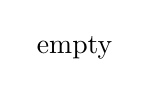
\begin{tikzpicture}
	\node at (0,0){empty};
	\end{tikzpicture}
	\caption{Classification of Machine Learning algorithms}
	\label{fig:classification_ml} 
\end{figure}

This thesis deals with Dynamic Programming for policy optimization. More specifically, policy iteration and value iteration are applied to a trajectory optimization problem. In a prior work on this topic, TRPO and A3C were applied to a 2D trajectory optimization problem~\cite{Zuern2017}. Both algorithms deal with the complete environment, i.e. the glider dynamics and the stochastic wind distribution, at the same time. Whereas the wind distribution is unknown a priori, the glider dynamics are well known. Therefore, a DP algorithm can be applied to any scenario with calm air. The resulting optimal policy $\pi^*_{\text{calm}}$ then can be used as a starting point for TRPO in scenarios with unknown wind conditions.
\begin{figure}[h]
	\centering
	\tikzsetnextfilename{mdp_algos}
	\begin{tikzpicture}
	\node (rect) at (-5,7) [draw, fill = UniSHellblau]{Policy Optimization};
	\node (rect) at (5,7) [draw, fill = UniSHellblau]{Dynamic Programming};
	\node at (-7,4) {Evolution};
	\node at (-3,4) {Policy Gradients};
	\node at (3,4) {Policy Iteration};
	\node at (7,4) {Value Iteration};
	\node at (5,2) {Q-Learning};
	\node at (0,1) {Actor-Critic Methods};
	\draw (-5.5,6.5) -- (-6.5,4.5);
	\draw (-4.5,6.5) -- (-3,4.5);
	\draw (-2.5,3.5) -- (-0.5,1.5);
	\draw (5.5,6.5) -- (6.5,4.5);
	\draw (4.5,6.5) -- (3,4.5);
	\draw (2.5,3.5) -- (0.5,1.5);
	\draw (6.5,3.5) -- (5.5,2.5);
	\draw [dashed,line width = 3pt] (0,2) -- + (0,5);
	
	\draw [draw=gray, line width=1.5pt] (1.3,3.5) rectangle (8.7,4.5); 
	\end{tikzpicture}
	\caption{MDP solution methods, adopted from~\cite{Schulman2016}]}
	\label{fig:RLmethods} 
\end{figure}

Dynamic programming is a general term, that is used for algorithms that solve a specific type of problem. Those problems can be decomposed into subproblems and solved by composing the solutions of those subproblems. If the subproblems are very similar, the solution of one subproblem can be used to calculate another one. In such cases, dynamic programming is applicable. In MDPs, these subproblems are similar in the sense that the Bellman Expectation Equation and the Bellman Optimality Equation hold true in all states, i.e. each state (and action) value is connected to its successor values by the Bellman Equations.

Also, the optimal action is found in all states the same way, as can be seen in section \ref{sec:PI}. If the algorithm is successful, the policy is optimal according to section \ref{sec:optimality}. Unlike with TRPO, optimization is not done through sampling complete trajectories, but by iterating the state-values and policy for each state independently. After one sweep over the state space, the value function and policy are updated and the process is repeated.\bigbreak

In theory, starting TRPO or A3C with a policy that is already optimal with respect to the scenario in calm air should accelerate training with updrafts because the information about how to behave in a situation with no wind is already incorporated in the policy.

\subsection{Approximate Dynamic Programming}

Dynamic programming has been utilized to solve problems in various disciplines since its invention. Most of the applications were in finance, computer science and control theory. The latter is also the topic of this thesis. Unfortunately, the descriptions of the relationship between RL and DP vary from discipline to discipline and seem inconsistent at first. Therefore, this section contains some information about important keywords and methods in DP and RL and tries to bring the different viewpoints of control theory, computer science and finance together. For each discipline, the relevant nomenclature is shown and some sources containing further information are given. Then, the seemingly inconsistent viewpoints are brought together.

The term Approximate Dynamic Programming (ADP) \nomenclature[A]{ADP}{Approximate Dynamic Programming} often comes up in the context of machine learning. (Daran tippe ich gerade, mir geht es vor allem um den Aufbau von Kapitel 2.)

\subsection{Types of Dynamic Programming Algorithms}

\subsubsection{Policy Evaluation}
\label{subsection:policy_evaluation}

In Policy Evaluation, the goal is to find an approximation of the value function $V_\pi$ that corresponds to a given policy $\pi$. The value of a state is defined as the expected total return from that state onwards until the episode terminates. Obviously, the expectation in equation \ref{eq:bellman_exp} depends on the actions that are taken at each step and therefore on the policy that is evaluated. The state value that corresponds to a specific policy $\pi$ is denoted by $V_\pi(s)$.

\begin{align}
V_\pi(s_t)&=\mathbb{E}[G_t|s_t=s]\\ &= \mathbb{E}\left[ \sum_{k=0}^{T-t-1}\gamma^k r_{t+k+1}|s_t=s\right] \\
&=\mathbb{E}[r_{t+1}+\gamma^1 r_{t+2}+\gamma^2 r_{t+3}+\gamma^3 r_{t+4}+...+\gamma^{T-t-1}r_T|s_t=s]
\label{eq:bellman_exp}
\end{align}

With a stochastic discrete policy, equation \ref{eq:bellman_exp} becomes

\begin{equation}
V_\pi(s_t)=\sum_{a}\pi(a|s)(\mathcal{R}(s,a)+\gamma V_\pi(s'))
\label{eq:bellman_exp_discrete_policy}
\end{equation}

Recall the definition of a state value $V(s) = \mathbb{E}[G_t|s_t=s]$ from Eq. \ref{eq:state_value_fun}. This equation can be used as a mapping to update the value of $s_t$ with the expected return according to the current policy.

\begin{equation}
V_\pi(s_t) \mathrel{\reflectbox{\ensuremath{\mapsto}}} \mathbb{E}[ \sum_{k=0}^{T-t-1}\gamma^k r_{t+k+1}|s_t=s]
\label{eq:bellman_exp_update}
\end{equation}

In Eq. \ref{eq:bellman_exp}, all terms expect the first one can be replaced by the expected return from $s_{t+1}$ onwards:

\begin{align}
V_\pi(s_t) \mathrel{\reflectbox{\ensuremath{\mapsto}}} 
&\;\mathbb{E}[r_{t+1}+\gamma G_{t+1}|s_t=s]\\
=&\;r_{t+1}+\gamma V_\pi(s_{t+1})
\label{eq:bellman_exp_update_bootstrapped}
\end{align}

With a discrete stochastic policy, equation \ref{eq:bellman_exp_update_bootstrapped} becomes


\begin{equation}
V_{\pi}(s_t) \mathrel{\reflectbox{\ensuremath{\mapsto}}} \sum_{a}\pi(a|s)(r_t+\gamma V_\pi(s'))
\label{eq:bellman_exp_update_discrete}
\end{equation}

In a state space with a finite set of states $\mathcal{S}$, writing down Eq. \ref{eq:bellman_exp_update_discrete} for each state results in a system of $|\mathcal{S}|$ linear equations that can be solved for $V(s)$. If the number of states is very large, this is not very efficient. 

Instead, \ref{eq:bellman_exp} is usually solved iteratively. The simplest way is to perform a one step lookahead from each state to get $r_t$ and $V(s_{t+t})$ from the current estimate of the state value function. Once all values are calculated, the values of all states are updated simultaneously \footnote{There are variants of Policy Iteration, where the updates are performed asynchronously. This means that, for example, all neighbors of a terminal state are updated first. After that, the states, that lie next to these states, are updated, and so on. They usually converge faster, but at the expense of implementation complexity.}. Unlike other RL-algorithms, the state values are not updated along a trajectory. Instead, each state is updated independently.

Each set of state values approximates the true value function of the problem better than the previous set of estimates. Every state value converges to the true state value under the given policy. It is not efficient to wait until the values have fully converged, i.e. the true value function $V_\pi$ is reached. Instead the process is repeated until the maximum absolute change in values lies beneath a certain threshold $\epsilon_V$. This maximum absolute change can be expressed by the supremum-norm $||(\cdot)||_\infty$ (c.f. section \ref{sec:contraction_mappings}). Algorithm \ref{algo:pe} shows a possible implementation of iterative policy evaluation. In practice, there can be an upper bound for the number of evaluation steps.

\begin{equation}
||V_{k}-V_{k-1}||_\infty<\epsilon_V
\label{eq:pe_stopping_criterion}
\end{equation}

\begin{algorithm}[hbt]
	
	\begin{algorithmic}[0] % 1 to show code line numbers
		
		\Function{Policy Evaluation}{}
		\State Initialize $V(s) = 0 \; \forall \; s \in \mathcal{S}$ and load policy $\pi$.
		\While {true}
		\ForAll{$s \in \mathcal{S}$}
		\State $V_{\pi,new}(s) \mathrel{\reflectbox{\ensuremath{\mapsto}}} r+\gamma V_ {\pi,old}(s')$
		\EndFor
		\If {$||V_{new}-V_{old}||_\infty \leq \epsilon_V$}
		\State break
		\EndIf
		\EndWhile
		\EndFunction
	\end{algorithmic}
	\caption{Iterative policy evaluation}
	\label{algo:pe}
\end{algorithm}

\subsubsection{Policy Iteration}
\label{sec:PI}
Policy iteration is an iterative way to calculate an estimate of the optimal policy of an MDP. Starting with an arbitrary policy and value function, one iteration of policy evaluation is performed to get an estimate of $V_\pi$. After that, after that, the policy is replaced by the greedy policy w.r.t. to the new value function estimate $V_\pi$. This alternating process of Policy Evaluation and Policy Improvement is repeated until the policy is satisfactory.

\begin{equation}
a_{\text{greedy}}(s_t) = \underset{a}{\text{argmax}}[Q(s_t,a_t)]
\end{equation}

For a deterministic, greedy policy $\pi_{\text{greedy}}$, this yields:

\begin{align}
\pi(a_{\text{greedy}}|s_t)&=\mathbb{P}[a_t=a_{\text{greedy}}(s_t)|s_t] \\ &=1
\end{align}

and for a stochastic policy $\pi$:

\begin{equation}
\mathbb{E}[\pi(a_t | s_t)] \mathrel{\reflectbox{\ensuremath{\mapsto}}} a_{\text{greedy}}
\end{equation}

As mentioned in subsection \ref{subsection:policy_evaluation}, each policy evaluation step usually ends if the maximum difference between two subsequent values of the same state are sufficiently close.

There is a version of Policy Iteration where only one value update is done before updating the policy. This algorithm is called Optimistic Policy Iteration (OPI). Although the first estimate of the value function is only a rough approximation, OPI also converges to the optimal value function and policy. The following diagram illustrates the policy iteration scheme.

\begin{equation*}
\pi_0 \overset{evaluate}{\longrightarrow} V_1 \overset{improve}{\longrightarrow} \pi_1 \overset{evaluate}{\longrightarrow} V_2 \overset{improve}{\longrightarrow} \pi_2 \overset{evaluate}{\longrightarrow} ... \overset{evaluate}{\longrightarrow} V_* \overset{improve}{\longrightarrow} \pi_*
\label{eq:pi_scheme}
\end{equation*}

Another way to picture policy iteration is shown in figure \ref{fig:PI_triangle}. Every PI-step brings the Value Function $V(s)$ closer to $V_*(s)$ and the policy $\pi$ closer to $\pi_*$.

Policy iteration can be seen as two competing processes. On one hand, every policy evaluation step changes $v$, which leads to a change in the greedy policy. The previous greedy policy is therefore no longer greedy after the evaluation step. On the other hand, every policy improvement step makes the policy greedy w.r.t the current value function. This typically changes the value function, so the value function before the policy update is no longer the correct one (cf. \cite[section~4.6]{SuttonBarto2018}).

\begin{figure}[htb]
	\centering
	\tikzsetnextfilename{pi_sketch}
		\begin{tikzpicture}
			\draw[name path=v_pi] (10,0) -- node[above,rotate=-16.699]{$v=v_\pi$} +(-10,3);
			\draw[name path=pi_greedy] (10,0) -- node[below,rotate=16.699]{$\pi=greedy(v)$} +(-10,-3);
			\node at (10.6,0) {$\pi_*,v_*$};
			\fill[black] (0.6,-1) circle (3pt);
			\node at (0.2,-1) {$\pi_0$};
			\fill[black] (9.5,0) circle (1pt);
			\fill[black] (9.2,0) circle (1pt);
			\fill[black] (8.9,0) circle (1pt);
			\draw[draw=none,name path=pe1] (0,-3) -- +(1.8,6);
			\draw[-latex,line width = 1.5pt,name intersections={of=pe1 and v_pi,by={v_1}}] (0.6,-1) -- (v_1);
			\draw[draw=none,name path=pi1] (v_1) -- +(1.8,-6);
			\draw[-latex,line width = 1.5pt,name intersections={of=pi1 and pi_greedy,by={pi_1}}] (v_1) -- (pi_1);
			\draw[draw=none,name path=pe2] (pi_1) -- +(1.2,4);
			\draw[-latex,line width = 1.5pt,name intersections={of=pe2 and v_pi,by={v_2}}] (pi_1) -- (v_2);
			\draw[draw=none,name path=pi2] (v_2) -- +(1.2,-4);
			\draw[-latex,line width = 1.5pt,name intersections={of=pi2 and pi_greedy,by={pi_2}}] (v_2) -- (pi_2);
			\draw[draw=none,name path=pe3] (pi_2) -- +(1.2,4);
			\draw[-latex,line width = 1.5pt,name intersections={of=pe3 and v_pi,by={v_3}}] (pi_2) -- (v_3);
			\draw[draw=none,name path=pi3] (v_3) -- +(1.2,-4);
			\draw[-latex,line width = 1.5pt,name intersections={of=pi3 and pi_greedy,by={pi_3}}] (v_3) -- (pi_3);
			\draw[draw=none,name path=pe4] (pi_3) -- +(0.6,2);
			\draw[-latex,line width = 1.5pt,name intersections={of=pe4 and v_pi,by={v_4}}] (pi_3) -- (v_4);
			\draw[draw=none,name path=pi4] (v_4) -- +(0.6,-2);
			\draw[-latex,line width = 1.5pt,name intersections={of=pi4 and pi_greedy,by={pi_4}}] (v_4) -- (pi_4);
			\draw[draw=none,name path=pe5] (pi_4) -- +(0.6,2);
			\draw[-latex,line width = 1.5pt,name intersections={of=pe5 and v_pi,by={v_5}}] (pi_4) -- (v_5);
			\draw[draw=none,name path=pi5] (v_5) -- +(0.6,-2);
			\draw[-latex,line width = 1.5pt,name intersections={of=pi5 and pi_greedy,by={pi_5}}] (v_5) -- (pi_5);

			\node[blue] at (0.8,-2) {$\pi_0$};
			\fill[blue] (1.2,-2) circle (3pt);
			\draw[draw=none,name path=opiline] (1,-1.5) -- + (10,3);
			\draw[draw=none,name path=ope1] (1.2,-2) -- + (0.6,2);
			\draw[blue,-latex,line width = 1.5pt,name intersections={of=ope1 and opiline,by={ope_1}}] (1.2,-2) -- (ope_1);
			\draw[draw=none,name path=opi1] (ope_1) -- +(0.6,-2);
			\draw[blue,-latex,line width = 1.5pt,name intersections={of=opi1 and pi_greedy,by={opi_1}}] (ope_1) -- (opi_1);
			\draw[draw=none,name path=ope2] (opi_1) -- +(0.6,2);
			\draw[blue,-latex,line width = 1.5pt,name intersections={of=ope2 and opiline,by={ope_2}}] (opi_1) -- (ope_2);
			\draw[draw=none,name path=opi2] (ope_2) -- +(0.6,-2);
			\draw[blue,-latex,line width = 1.5pt,name intersections={of=opi2 and pi_greedy,by={opi_2}}] (ope_2) -- (opi_2);
			\draw[draw=none,name path=ope3] (opi_2) -- +(0.6,2);
			\draw[blue,-latex,line width = 1.5pt,name intersections={of=ope3 and opiline,by={ope_3}}] (opi_2) -- (ope_3);
			\draw[draw=none,name path=opi3] (ope_3) -- +(0.6,-2);
			\draw[blue,-latex,line width = 1.5pt,name intersections={of=opi3 and pi_greedy,by={opi_3}}] (ope_3) -- (opi_3);
			\draw[draw=none,name path=ope4] (opi_3) -- +(0.6,2);
			\draw[blue,-latex,line width = 1.5pt,name intersections={of=ope4 and opiline,by={ope_4}}] (opi_3) -- (ope_4);
			\draw[draw=none,name path=opi4] (ope_4) -- +(0.6,-2);
			\draw[blue,-latex,line width = 1.5pt,name intersections={of=opi4 and pi_greedy,by={opi_4}}] (ope_4) -- (opi_4);
			\draw[draw=none,name path=ope5] (opi_4) -- +(0.6,2);
			\draw[blue,-latex,line width = 1.5pt,name intersections={of=ope5 and opiline,by={ope_5}}] (opi_4) -- (ope_5);
			\draw[draw=none,name path=opi5] (ope_5) -- +(0.6,-2);
			\draw[blue,-latex,line width = 1.5pt,name intersections={of=opi5 and pi_greedy,by={opi_5}}] (ope_5) -- (opi_5);
			\draw[draw=none,name path=ope6] (opi_5) -- +(0.6,2);
			\draw[blue,-latex,line width = 1.5pt,name intersections={of=ope6 and opiline,by={ope_6}}] (opi_5) -- (ope_6);
			\draw[draw=none,name path=opi6] (ope_6) -- +(0.6,-2);
			\draw[blue,-latex,line width = 1.5pt,name intersections={of=opi6 and pi_greedy,by={opi_6}}] (ope_6) -- (opi_6);
			\draw[draw=none,name path=ope7] (opi_6) -- +(0.6,2);
			\draw[blue,-latex,line width = 1.5pt,name intersections={of=ope7 and opiline,by={ope_7}}] (opi_6) -- (ope_7);
			\draw[draw=none,name path=opi7] (ope_7) -- +(0.6,-2);
			\draw[blue,-latex,line width = 1.5pt,name intersections={of=opi7 and pi_greedy,by={opi_7}}] (ope_7) -- (opi_7);
			\draw[draw=none,name path=ope8] (opi_7) -- +(0.6,2);
			\draw[blue,-latex,line width = 1.5pt,name intersections={of=ope8 and opiline,by={ope_8}}] (opi_7) -- (ope_8);
			\draw[draw=none,name path=opi8] (ope_8) -- +(0.6,-2);
			\draw[blue,-latex,line width = 1.5pt,name intersections={of=opi8 and pi_greedy,by={opi_8}}] (ope_8) -- (opi_8);
			\draw[draw=none,name path=ope9] (opi_8) -- +(0.6,2);
			\draw[blue,-latex,line width = 1.5pt,name intersections={of=ope9 and opiline,by={ope_9}}] (opi_8) -- (ope_9);
			\draw[draw=none,name path=opi9] (ope_9) -- +(0.6,-2);
			\draw[blue,-latex,line width = 1.5pt,name intersections={of=opi9 and pi_greedy,by={opi_9}}] (ope_9) -- (opi_9);
			\draw[draw=none,name path=ope10] (opi_9) -- +(0.6,2);
			\draw[blue,-latex,line width = 1.5pt,name intersections={of=ope10 and opiline,by={ope_10}}] (opi_9) -- (ope_10);
			\draw[draw=none,name path=opi10] (ope_10) -- +(0.6,-2);
			\draw[blue,-latex,line width = 1.5pt,name intersections={of=opi10 and pi_greedy,by={opi_10}}] (ope_10) -- (opi_10);
			
		\end{tikzpicture}
	\caption{The policy iteration algorithm (adopted from~\cite[section~4.6]{SuttonBarto2018}}
	\label{fig:PI_triangle}
\end{figure}

The black arrows in Fig. \ref{fig:PI_triangle} refer to a policy iteration algorithm, that calculates $v_\pi$ exactly in every evaluation step. This typically takes long for one iteration, but requires less iterations than optimistic policy iteration. The latter is what the blue arrows refer to. Each policy evaluation step only yields a rough estimate of $v_\pi$ and takes less time than exact evaluation. OPI however usually takes more iterations than exact PI.

The performance of both algorithms on the trajectory optimization problem is compared in chapter \ref{chapter6}. \bigbreak

In a discrete MDP, there is a finite number of states and actions. At each state $s \in \mathcal{S}$, the agent can choose the action $a$ from a set $\mathcal{A}$ of possible actions. In such a scenario, there exist $|\mathcal{A}|^{|\mathcal{S}|}$ different policies. It therefore takes $|\mathcal{A}|^{|\mathcal{S}|}$ iterations to find the optimal policy assuming no policy occurs twice. If that was the case, this policy would have to occur in two subsequent iterations and therefore be the fixed point $\pi_*$ of the policy sequence generated by PI.

As the results in chapter \ref{chapter6} show, PI converges much faster in practice than the upper bound $|\mathcal{A}|^{|\mathcal{S}|}$ may suggest. Algorithm \ref{algo:gpi} shows one way to implement generalized policy iteration. The algorithm alternates between PE and policy improvement until none of the actions change from one iteration to the next. The pseudo code for optimistic policy iteration can be found in algorithm \ref{algo:opi} in appendix \ref{appendix_D}.

\begin{algorithm}[hbt]
	\begin{algorithmic}[0] % 1 to show code line numbers
		\Function{Generalized Policy Iteration}{}
		\State Initialize $V(s) = 0 \; \forall \; s \in \mathcal{S}$
		\State Load arbitrary initial policy $\pi_0$.
		\State Initialize $m$,\;$\epsilon_V$
		\While {true}			
		\Function{Policy Evaluation}{}
		\While {true}
		\ForAll{$s \in \mathcal{S}$}
		\State $V_{\pi,new}(s) \mathrel{\reflectbox{\ensuremath{\mapsto}}} r+\gamma V_ {\pi,old}(s')$
		\EndFor
		\If {$||V_{new}-V_{old}||_\infty \leq \epsilon_V$}
		\State break
		\EndIf
		\EndWhile
		\EndFunction
		\Function{Policy Improvement}{}
		\ForAll{$s \in \mathcal{S}$}
		\State sample $m$ actions $a_n(s)$
		\ForAll {$a_n$}
		\State $Q(s,a_n) = r + \gamma V(s')$
		\EndFor
		\State $a_{greedy}(s)=\underset{a_n}{\text{argmax}}[Q(s,a_n)]$
		\EndFor
		\EndFunction
		\State
		\State train policy on $a_{greedy,new}$ to obtain $\pi_{new}$
		\If {$||a_{greedy,new}-a_{greedy,old}||_\infty = 0$}
		\State break
		\EndIf
		
		\EndWhile
		\State
		\EndFunction
	\end{algorithmic}
	\caption{Generalized policy iteration}
	\label{algo:gpi}
\end{algorithm}

\subsubsection{Value Iteration}
\label{subsection:VI}
Value iteration is similar to policy iteration, but instead of calculating a new policy at each iteration step, the state values $V(s)$ are directly updated with the maximum possible successor value that is achievable starting from $s$. This yields a sequence of value functions, each one being a better estimate of $V_*$ than its predecessor. Each of the intermediate value functions is abstract in so far as there does not have to exist an explicit policy corresponding to it (c.f. \cite[lecture~3]{Silver2015}). In a possibly discounted MDP with a deterministic environment, the update rule for each state value can be seen in equation \ref{eq:value_iteration_update}.

\begin{equation}
V(s_t) \mathrel{\reflectbox{\ensuremath{\mapsto}}} 
\underset{a}{\text{max}}[r_{t+1}+\gamma V(s_{t+1})|s_t=s]
\label{eq:value_iteration_update}
\end{equation}

In principle, this is equivalent to synchronous OPI, where after one state value update at each state, the policy is replaced by the greedy policy with respect to the new value function. The only difference is, that value iteration does not output an intermediate policy at each iteration. Instead, it only iterates value functions. 

\begin{equation*}
V_1 \longrightarrow V_2 \longrightarrow V_3 \longrightarrow ... \longrightarrow  V_*
\label{eq:vi_scheme}
\end{equation*}

In practice, a stopping criterion is introduced to limit calculation time. In this work, iteration is stopped if $||V_{k}-V_{k-1}||_\infty<\epsilon_V$, identical to equation \ref{eq:pe_stopping_criterion}. The last iterate $V_n$ is considered an approximation of $V_*$. If $V_n$ is close enough to the true optimal value function $V_*$, the (approximately) optimal policy can be calculated in the end by acting greedily with respect to $V_n$. Recall that, if Value Iteration is stopped too early, there might not even be a real policy that corresponds to the last value function iterate $V_n$ \cite[lecture~3]{Silver2015}. A possible implementation of value iteration is shown in algorithm \ref{algo:vi}.

\begin{algorithm}[hbt]
	\begin{algorithmic}[0] % 1 to show code line numbers
		\Function{Value Iteration}{}
		\State Initialize $V(s) = 0 \; \forall \; s \in \mathcal{S}$
		\State Initialize $m$,\;$\epsilon_V$
		\While {true}	
		\ForAll {$s \in \mathcal{S}$}
		\State sample $m$ actions $a_n(s)$
		\ForAll {$a_n$}
		\State $Q(s,a_n) = r + \gamma V(s')$
		\EndFor		
		\State $V_{new}(s)=\underset{a_n}{\text{max}}[Q(s,a_n)]$
		\EndFor
		\If {$||V_{new}-V_{old}||_\infty \leq \epsilon_V$}
		\State break
		\EndIf
		\EndWhile
		\Function{Policy Improvement}{}
		\ForAll{$s \in \mathcal{S}$}
		\State sample $m$ actions $a_n(s)$
		\ForAll {$a_n$}
		\State $Q(s,a_n) = r + \gamma V(s')$
		\EndFor
		\State $a_{greedy}(s)=\underset{a_n}{\text{argmax}}[Q(s,a_n)]$
		\EndFor
		\EndFunction
		\State train policy on the latest $a_{greedy,new}$ to obtain an estimate of $\pi_*$
		\EndFunction
	\end{algorithmic}	
	\caption{Value iteration}
	\label{algo:vi}
\end{algorithm}

\subsection{The Contraction Mapping Theorem}
\label{sec:contraction_mappings}
A contraction mapping $f: M \to M$ on a metric space $M$ has the following property:
\begin{equation}
|f(x_1)-f(x_2)| \leq \gamma |x_1-x_2|
\end{equation}

with $x_1,x_2 \in M$ and $\gamma \in [0,1)$. In this context,  $|(\cdot)|$ denotes an arbitrary metric on $M$.

The term contraction reflects the fact that, graphically speaking, a contraction mapping reduces the distance between $x_1$ and $x_2$.

\subsubsection*{Discounted MDPs}

Policy Evaluation in discounted MDPs is a contraction mapping. This result can be obtained in few steps. The mapping in equation \ref{eq:bellman_exp_update_discrete} and \ref{eq:bellman_operator_discounted} is known as the \textit{Bellman Operator}. It maps from a state value function to a state value function. If the Bellman Operator is applied multiple times, this can be expressed by $T^n(v)$.

\begin{equation}
T_\pi(v(s'))=\mathcal{R}_\pi+\gamma \mathcal{P}_\pi v(s')
\label{eq:bellman_operator_discounted}
\end{equation}

If the Bellman Operator is applied to two state value functions $V_1(s)$ and $V_2(s)$, it reduces the distance between the two in value function space. This distance can be expressed by the supremum norm, which is defined as follows:

\begin{equation}
||V||_\infty = \max_{s \in \mathcal{S}} |V(s)|
\end{equation}

The supremum norm of $V_1 - V_2$ is therefore

\begin{equation}
||V_1(s) - V_2(s)||_\infty = \max_{s \in \mathcal{S}} |V_1(s)-V_2(s)|
\end{equation}

which is the biggest absolute difference of values of the same state in the state space. If the Bellman Operator is applied to both $V_1$ and $V_2$, the contraction property proof is straightforward. For simplicity, the arguments of $V_1(s)$ and $V_2(s)$ are omitted in the following equations.
\begin{align}
||T_\pi(V_1)-T_\pi(V_2)||_\infty &= ||(\mathcal{R}_\pi+\gamma \mathcal{P}_\pi V_1)-(\mathcal{R}_\pi+\gamma \mathcal{P}_\pi V_2)||_\infty \label{eq:4.15}\\
&=||\gamma\; \mathcal{P}_\pi\;(V_1 - V_2)||_\infty \label{eq:4.16}\\
&\leq ||\gamma \mathcal{P}_\pi ||V_1 - V_2||_\infty ||_\infty \label{eq:4.17} \\
&\leq ||\gamma ||V_1 - V_2||_\infty ||_\infty \label{eq:4.18}\\
&=\gamma ||V_1 - V_2||_\infty \label{eq:4.19}
\end{align} 

Whenever $s'$ happens to be the state where $V_1$ and $V_2$ differ the most, equality holds in line \ref{eq:4.17}. If not, applying the supremum norm to $V_1(s')-V_2(s')$ increases the value of the expression. $\mathcal{P}_\pi$ must always be smaller than or equal to one. Similar to line \ref{eq:4.17}, equality in line \ref{eq:4.18} holds only if $\mathcal{P}_\pi=1$. Replacing $\mathcal{P}_\pi$ by one in line \ref{eq:4.17} yields line \ref{eq:4.18}. The left side of line \ref{eq:4.15} must thus be less than line \ref{eq:4.19} which proves the contraction property of the Bellman Operator in discounted MDPs.

\subsubsection*{Undiscounted MDPs}

An MDP, where the discount factor $\gamma$ is one, is called an undiscounted MDP. In such an MDP, the Bellman Operator looks like in equation \ref{eq:bellman_undiscounted}.

\begin{equation}
T_\pi(v(s))=\mathcal{R}_\pi + \mathcal{P}_\pi V(s')
\label{eq:bellman_undiscounted}
\end{equation}

If $\gamma$ is one, the above proof of the contraction property does not hold anymore. It can however be proven, that the Bellman Operator still contracts. In the undiscounted case, this takes more than one step. Equation \ref{eq:n-step-contraction} shows the n-step contraction property. For simplicity, the index $\pi$ and the argument $s$ are omitted.

\begin{equation}
||T^{(n)}(V_1)-T^{(n)}(V_2)||_\infty \leq ||V_1-V_2||_\infty
\label{eq:n-step-contraction}
\end{equation}

Equation \ref{eq:n-step-contraction} means, that applying the Bellman Operator n times to two value functions brings them closer together in value function space. As a result, the Bellman Operator also leads to $V_1 \approx V_2$ eventually also in undiscounted MDPs.

A proof, that policy iteration and value iteration also converge in undiscounted MDPs, can be found in \cite{},\cite{} and \cite{} (die trage ich in der nächsten Fassung noch ein).

\section{Exploiting the specific Problem Structure}

According to \cite{Powell2007ADP}, there is no such thing as a universal dynamic programming algorithm that is capable of solving various problems efficiently. Instead, making use of the structure of a problem is often vital in order to reduce computation time or make DP feasible in the first place. The following paragraph illustrates how this can be done in the case of path planning through value iteration.

In numerics, making use of new information as soon as it is available often reduces calculation time significantly. In value iteration, this can mean to update a state value as soon as a new value has been calculated. This way, subsequent calculations can make use of more recent data than in the case of synchronous updates\footnote{Recall that, in synchronous DP, the state values are updated at the same time after one complete sweep over the state space. If the start state $s_0$ is 50 steps away from the target state $s_T$, it takes 50 iterations (i.e. complete sweeps over the state space) to find a trajectory from $s_0$ to $s_T$.}. The most efficient way to exploit the problem structure in this work (cf. \ref{chapter5}) is to go backwards through the state space. The states directly next to the terminal states are updated first and simultaneously. After that, the layer\footnote{In this context, one layer is one set of points that have the same x-coordinate. This set forms a vertical "layer" of states that have the same distance to the goal.} next to these states is updated and so on. This way, the final reward can propagate to the start state in one iteration, i.e. one backward pass through the state space. As the value iteration algorithm in this work also considers movement (i.e. movement away from the goal), it typically takes about a thi